\chapter{Future Work}\label{future}

\section{Improving the xG Model}
The revised analysis points to several improvements to the model itself:
\begin{itemize}
    \item \textbf{Finer play patterns.} Counter attacks convert at 16.3\%, far above any other play pattern, but the Regular/Non Regular grouping used here hides them. Keeping counter attacks, and perhaps corners, as separate categories should make the play pattern useful.
    \item \textbf{More of the freeze frame.} The model uses only two counts of opponents. The positions of the nearest defenders, whether the goalkeeper is set, and the space in front of the shooter could all be derived from the same freeze frames.
    \item \textbf{Recalibration by level.} A pooled model transfers between the top European leagues, but not fully to a league of a different standard. A simple recalibration for each such league, using its own shots, could be tested.
    \item \textbf{More seasons.} With more complete seasons, the analysis of teams and leagues could be extended to changes over time and to team strength.
\end{itemize}

\section{Beyond xG}
The work presented in this study forms a bedrock for future metrics. An important question that arises within the minds of those who actively follow xG models is\\

\begin{center}
\textit{\textbf{Why does an xG model not inculcate the shot technique used and the shot velocity?}}
\end{center}

The answer to this question serves as the provenance to a new metric. The reason why those two features are not utilized is that an xG model is a \textit{pre-shot} analysis. It simply measures a player/team's intelligence through understanding the kind of positions they get into during a football match and make the art of scoring easier. Therefore, to utilize a player's capability as a striker and a finisher, a metric to understand \textit{post-shot} analysis needs to be created. This metric is called, Expected Goals on Target (xGOT). The following points need to be considered to develop the xGOT metric

\begin{itemize}
    \item Placement of the shot
    \item Technique Used
    \item Velocity of the Shot
    \item The xG value of the Shot
\end{itemize}

A poor finisher could be hypothesised as one, who places a high xG valued shot in an easy to save position. This could be an example of how xGOT can be utilised to quantify player ability. Furthermore, xGOT can also be used to quantify the ability of the Goal Keeper saving the shot. A good Goal Keeper can be hypothesised as one who consistently saves football shots with high xGOT values.

Figure \ref{shotplace} highlights different coordinates of a goal for reference to shot placement. A good finisher can be hypothesised as one who places the shot aimed close to the four corners. Similarly a good goal keeper is one who consistently saves shots aimed at these four corners. 

\begin{figure}[!h]
    \centering
    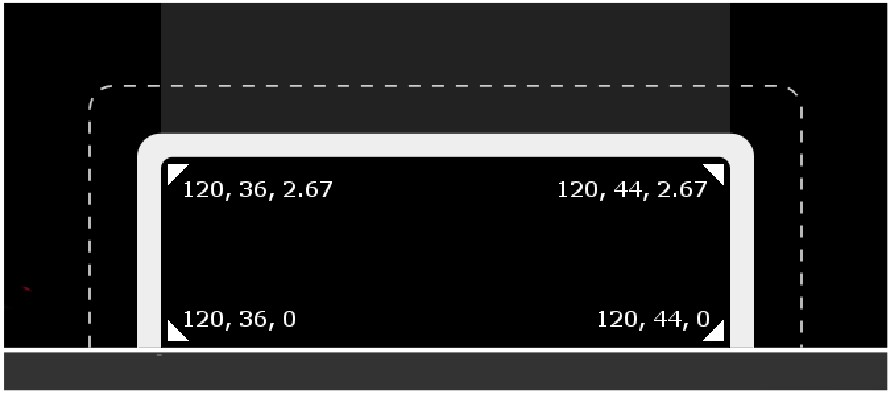
\includegraphics[scale=0.70]{images/shotplace.jpg}
    \caption{Shot Placement}
    \label{shotplace}
\end{figure}

Another metric that is derived from xG is Expected Goals Against (xGA). This metric provides perspective in how any given team allows others to create chances against themselves. A defensively good footballing team would allow others to create chances with less xG values.

A third metric that can be developed is one that analyses off-ball positioning first mentioned by author \citeauthor{spearman2018beyond} in \cite{spearman2018beyond}. This study aims at analysing the positioning of players and determining how likely they are to score while positioned without the ball highlighted in figure \ref{offball}.

\begin{figure}[!h]
    \centering
    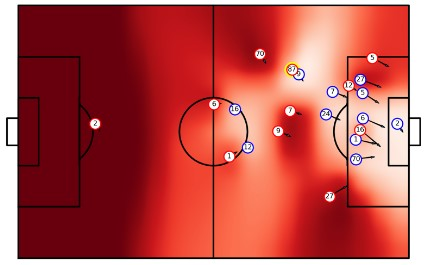
\includegraphics[scale=1, angle=90]{images/spearman.jpg}
    \caption{Off Ball Scoring}
    \label{offball}
\end{figure}




